% !TeX program = xelatex
% !TeX encoding = UTF-8
% !TeX spellcheck = en_US
% !BIB program = biber
%% 
%% The above lines help editors like TeXstudio to automatically choose the right tools
%% to compile your LaTeX source file. If your tool does not support these magic comments,
%% you will need to make appropriate manual choices.
%% 
%% You can safely use "pdflatex" instead of "xelatex" if you prefer the pdfLaTeX toolchain.
%% However, pdfLaTeX will not be able to deliver the professional font experience that you
%% will get with XeLaTeX. You can also safely use "lualatex" instead of "xelatex" while
%% preserving the professional font experience if you prefer the LuaLaTeX toolchain.
%% 
%% _Important_: These magic comments should be on the first lines of your source file.
%% 
%%%%%%%%%%%%%%%%%%%%%%%%%%%%%%%%%%%%%%%%%%%%%%%%%%%%%%%%%%%%%%%%%%%%%%%%%%%%%%%%

%%%%%%%%%%%%%%%%%%%%%%%%%%%%%%%%%%%%%%%%%%%%%%%%%%%%%%%%%%%%%%%%%%%%%%%%%%%%%%%%
%% 
%%            JJJJ   K                         K   UUUU         UUUU  
%%            JJJJ   KKKK                   KKKK   UUUU         UUUU  
%%            JJJJ   KKKKKK               KKKKKK   UUUU         UUUU  
%%            JJJJ      KKKKKK         KKKKKK      UUUU         UUUU  
%%            JJJJ         KKKKKK   KKKKKK         UUUU         UUUU  
%%            JJJJ            KKKKKKKKK            UUUU         UUUU  
%%    JJ     JJJJJ               KKK               UUUUU       UUUUU  
%%  JJJJJJJJJJJJJ    KKKKKKKKKKKKKKKKKKKKKKKKKKK    UUUUUUUUUUUUUUU   
%%    JJJJJJJJJ      KKKKKKKKKKKKKKKKKKKKKKKKKKK      UUUUUUUUUUU     
%% 
%% This is an example file for using the JKU LaTeX technical report template
%% for your seminar report.
%% 
%% Template created by Michael Roland (2023)
%% 
%%%%%%%%%%%%%%%%%%%%%%%%%%%%%%%%%%%%%%%%%%%%%%%%%%%%%%%%%%%%%%%%%%%%%%%%%%%%%%%%

%%%%%%%%%%%%%%%%%%%%%%%%%%%%%%%%%%%%%%%%%%%%%%%%%%%%%%%%%%%%%%%%%%%%%%%%%%%%%%%%
%% 
%% Document class: This is a koma-script article.
%% 
\documentclass[a4paper,oneside,10pt,ngerman,english]{scrartcl}
%% 
%% The comma-separated list in square brackets are class options.
%% Useful options that you might want to use:
%% 
%% Paper size:
%%  * a4paper ... A4 paper size
%% 
%% Optimize for single-sided or double-sided printing:
%%  * oneside ... single-sided
%%  * twoside ... double-sided
%% 
%% Base font size:
%%  * 10pt ... 10-pt font is used for normal text
%%  * 11pt ... 11-pt font is used for normal text
%% 
%% Define document languages (the last specified language becomes the document default
%% language):
%%  * ngerman ... German
%%  * english ... English
%%  * ...
%% 
%% Alternate document classes: The JKU report template supports the koma-script classes
%% `scrartcl', `scrreprt' and `scrbook'. The article class `scrartcl' is well-suited
%% for a typical seminar report. However, `scrbook' or `scrreprt' may be better
%% suited for longer reports since they permit structuring your work in chapters.
%%  
%% _Important_: The document class should be the first line of LaTeX code in your main
%% source file. Do not place anything but comments / magic comments above that line (unless
%% you really know what you are doing).
%% 
%%%%%%%%%%%%%%%%%%%%%%%%%%%%%%%%%%%%%%%%%%%%%%%%%%%%%%%%%%%%%%%%%%%%%%%%%%%%%%%%

%%%%%%%%%%%%%%%%%%%%%%%%%%%%%%%%%%%%%%%%%%%%%%%%%%%%%%%%%%%%%%%%%%%%%%%%%%%%%%%%
%% 
%% Treat input files as UTF-8 encoded. Make sure to always load this when you use pdfLaTeX
%% so that pdfLaTeX knows how to read and interpret characters in this source file.
%% 
\usepackage[utf8]{inputenc}
%% 
%%%%%%%%%%%%%%%%%%%%%%%%%%%%%%%%%%%%%%%%%%%%%%%%%%%%%%%%%%%%%%%%%%%%%%%%%%%%%%%%

%%%%%%%%%%%%%%%%%%%%%%%%%%%%%%%%%%%%%%%%%%%%%%%%%%%%%%%%%%%%%%%%%%%%%%%%%%%%%%%%
%% 
%% Use the JKU LaTeX technical report template for this document.
%% 
\usepackage[seminarreport,fancyfonts]{jkureport}
%% 
%% The comma-separated list in square brackets are theme options. Useful options that you
%% might want to use:
%% 
%% Document type:
%%  * phdthesis     ... PhD thesis.
%%  * mathesis      ... Master's thesis.
%%  * diplomathesis ... Diploma thesis.
%%  * bathesis      ... Bachelor's thesis.
%%  * seminarreport ... Seminar report.
%%  * techreport    ... Technical report.
%% 
%% Color scheme selection options:
%%  * JKU  ... Use JKU (gray) color scheme (this is the default if no scheme is selected).
%%  * BUS  ... Use Business School color scheme.
%%  * LIT  ... Use Linz Institute of Technology color scheme.
%%  * MED  ... Use MED faculty color scheme.
%%  * RE   ... Use RE faculty color scheme.
%%  * SOE  ... Use School of Education color scheme.
%%  * SOWI ... Use SOWI faculty color scheme.
%%  * TNF  ... Use TNF faculty color scheme.
%% 
%% Space-efficient monospace font options (requires XeTeX/LuaTeX):
%%  * compactmono   ... Use condensed fixed-width font everywhere.
%%  * nocompactverb ... Do not use condensed fixed-width font for verbatim and listings.
%% 
%% Style-breaking options:
%%  * noimprint      ... Do not insert imprint on title pages.
%%  * nojkulogo      ... Do not insert JKU & K logos on title pages.
%%  * capstitle      ... Set document title in capital letters.
%%  * nofancyfonts   ... Do not use custom TTF fonts with XeTeX/LuaTeX / supress pdfLaTeX warning.
%%  * equalmargins   ... Decrease the outer page margin to have both page margins of equal size
%%                       (the additional outer margin is intentional and to be used for
%%                       anotations; equalmargins also causes the text width to be
%%                       significantly larger than optimal for reading).
%% 
%% Experimental options:
%%  * mathastext ... Use standard document fonts (enhanced with symbols from Fira Math font
%%                   when using XeTeX/LuaTeX) in math mode.
%% 
%% Advanced options:
%%  * noautopdfinfo     ... Do not automatically try to add pdfinfo with hyperref from document
%%                          metadata fields.
%%  * logopath={<path>} ... Set the path where the theme can find its own logo resources. This
%%                          should typically be a relative path and the default is `./logos'.
%%  * fontpath={<path>} ... Set the path where the theme can find its own font resources. This
%%                          should typically be a relative path and the default is `./fonts'.
%% 
%% Hint: Boolean options can be used in the forms `option' or `option=true' the enable the
%% option and `nooption' or `option=false' to disable the option.
%% 
%%%%%%%%%%%%%%%%%%%%%%%%%%%%%%%%%%%%%%%%%%%%%%%%%%%%%%%%%%%%%%%%%%%%%%%%%%%%%%%%

%%%%%%%%%%%%%%%%%%%%%%%%%%%%%%%%%%%%%%%%%%%%%%%%%%%%%%%%%%%%%%%%%%%%%%%%%%%%%%%%
%% 
%% This is the place where you can load additional packages. If you want to load
%% a package `biblatex', you would use the command `\usepackage{biblatex}'.
%% 

\usepackage{csquotes}
\usepackage[backend=biber,citestyle=numeric,sortcites=true,maxcitenames=2,style=ACM-Reference-Format]{biblatex}
\setcounter{biburlnumpenalty}{100} %% reducing biburl* penalties typically improves URL placement in bibliography
\setcounter{biburllcpenalty}{100}
\setcounter{biburlucpenalty}{100}
\usepackage{todonotes}
\usepackage{import}
\usepackage{amsfonts}
\usepackage{float}
\usepackage{subfigure}
%\usepackage{acronym}

%% 
%%%%%%%%%%%%%%%%%%%%%%%%%%%%%%%%%%%%%%%%%%%%%%%%%%%%%%%%%%%%%%%%%%%%%%%%%%%%%%%%

%%%%%%%%%%%%%%%%%%%%%%%%%%%%%%%%%%%%%%%%%%%%%%%%%%%%%%%%%%%%%%%%%%%%%%%%%%%%%%%%
%% 
%% Bibliography data files.
%% 

\addbibresource{references.bib}

%% 
%%%%%%%%%%%%%%%%%%%%%%%%%%%%%%%%%%%%%%%%%%%%%%%%%%%%%%%%%%%%%%%%%%%%%%%%%%%%%%%%

\begin{document}
%%%%%%%%%%%%%%%%%%%%%%%%%%%%%%%%%%%%%%%%%%%%%%%%%%%%%%%%%%%%%%%%%%%%%%%%%%%%%%%%
%% 
%% Report information and title page
%% 

%% Command \title{title}: sets the title of your report
\title{Just Tell Me What You Like: Learning from Comparisons in Maze Environments}

%% Command \titleshort{short title}: sets an abbreviated version of the report title for page heads
%\titleshort{Optional space for your abbreviated title}

%% Command \subtitle{subtitle}: sets the subtitle for seminar/technical reports (not used for theses)
\subtitle{Technical Report}

%% Command \author{name}: sets the author's name; use \prefix{} and \suffix{} to add academic titles
%%   and suffixes, use \matno{} to add the immatriculation number
\author{Giovanni Filomeno \matno{12315325}}

%% Command \supervisor[number,gender]{name}: sets the name of the supervisor (where number optionally
%%   defines the rank of the supervisor (1-3) and gender specifies if the supervisor is male or female
%%   to adapt gener-specific terms in German)
%\supervisor[1]{\prefix{Prof. Dr.} Firstname~Lastname}
%\supervisor[2]{\prefix{Prof. Dr.} Firstname~Lastname}

%% Command \submissiondepartment{institute or department}: set the course or department that the thesis
%%   is submitted at
\submissiondepartment{Practical Work in AI (365.207)}

%% Command \date{YYYY-MM-DD}: set the day of submission (defaults to today)
%\date{2020-04-09}

%% Command \abstract{text}: set the document abstract on the title page
\abstract{This work explores how to train navigation policies in maze environments without relying on scalar rewards. Instead of assigning numeric scores to states or trajectories, pairwise preferences are collected, indicating which of two solutions is better, and used to directly optimize a policy. This approach is shown to successfully guide agents toward goals, even in complex mazes where greedy methods fail. The results highlight the importance of how preferences are defined, and suggest that direct preference-based methods offer a viable reward-free alternative for learning in structured environments.}

%% Command \keywords{text}: set the document keywords
%\keywords{Space for your comma-separated keywords}


%% Finally, print the title page using the above information:
\maketitle
%% 
%%%%%%%%%%%%%%%%%%%%%%%%%%%%%%%%%%%%%%%%%%%%%%%%%%%%%%%%%%%%%%%%%%%%%%%%%%%%%%%%

%%%%%%%%%%%%%%%%%%%%%%%%%%%%%%%%%%%%%%%%%%%%%%%%%%%%%%%%%%%%%%%%%%%%%%%%%%%%%%%%
%% 
%% Add a table of contents
%% 

%% Make sure to start the table of contents on a new odd page (odd is only relevant in twoside layout)
\cleardoubleoddpage
%% Print the table of contents
\tableofcontents

%% Make sure to start the list of acronyms on a new odd page (odd is only relevant in twoside layout)
%\cleardoubleoddpage
%% Include list of acronyms (optional and often not necessary)
%\import{./}{acronyms}

%% 
%%%%%%%%%%%%%%%%%%%%%%%%%%%%%%%%%%%%%%%%%%%%%%%%%%%%%%%%%%%%%%%%%%%%%%%%%%%%%%%%

%%%%%%%%%%%%%%%%%%%%%%%%%%%%%%%%%%%%%%%%%%%%%%%%%%%%%%%%%%%%%%%%%%%%%%%%%%%%%%%%
%% 
%% Abstract: Instead of an abstract on the title page (see \abstract{...}), you
%% sometimes want to add an abstract as its own unnumbered section.
%% 

%% (Optionally) let the abstract start on a new odd page (odd is only relevant in twoside layout)
\cleardoubleoddpage

\addsec{Abstract}

Preference-based methods have recently emerged as an effective alternative to traditional reinforcement learning, particularly when the design of a scalar reward function is difficult or unreliable. Among them, methods like Direct Preference Optimization (DPO) have demonstrated strong performance in aligning large language models with human feedback using a simple classification loss. In this project, this direct optimization approach has been adapted to a low-dimensional continuous control task: navigating maze environments using pairwise trajectory preferences.

Differently from prior applications that rely on a single scalar metric (e.g., sentiment or helpfulness), the environment considered here supports multiple interpretable criteria such as distance to the goal, wall proximity, and dead-end avoidance. A weighted scoring function has been proposed to combine these criteria, enabling the automatic generation of preferences between trajectory pairs. The resulting dataset is then used to train a policy by optimizing these pairwise preferences, bypassing the need for a manually engineered scalar reward signal at each step.

Experimental results indicate that this multi-parameter approach outperforms single-metric baselines, revealing a key insight: the success of preference-based learning is highly dependent on the quality and calibration of the preference signal itself. Poorly aligned scoring functions can prevent a policy from learning effectively, even when the preference dataset appears expressive.



%% 
%%%%%%%%%%%%%%%%%%%%%%%%%%%%%%%%%%%%%%%%%%%%%%%%%%%%%%%%%%%%%%%%%%%%%%%%%%%%%%%%

%%%%%%%%%%%%%%%%%%%%%%%%%%%%%%%%%%%%%%%%%%%%%%%%%%%%%%%%%%%%%%%%%%%%%%%%%%%%%%%%
%% 
%% Add your report sections ...
%% 

%% (Optionally) let the main sections start on a new odd page (odd is only relevant in twoside layout)
\cleardoubleoddpage

\section{Related Work}
\label{sec:relatedwork}

\subsection{Classical Reinforcement Learning vs Preference-Based Learning}

In classical reinforcement learning (RL), the agent learns a policy $\pi_\theta$ by maximizing the expected sum of rewards:
\[
\max_{\pi_\theta} \mathbb{E}_{x \sim \mathcal{D}, y \sim \pi_\theta} \left[ r(x, y) \right],
\]
where $r(x,y)$ is a scalar reward and $x$ the state/context. While this formulation is general, it critically depends on the design of $r(x, y)$, which is often sparse, delayed, or hard to specify in real-world environments \cite{christiano2017deep, ouyang2022training}. 

To circumvent this, preference-based learning removes the need for an explicit reward function, and instead learns from comparisons between trajectories $(y_w \succ y_l)$, leading to a loss of the form:
\[
\mathcal{L}_{\text{pref}}(r_\phi) = -\mathbb{E}_{(x, y_w, y_l) \sim \mathcal{D}} \log \sigma(r_\phi(x, y_w) - r_\phi(x, y_l)),
\]
where $\sigma$ is the logistic function, and $r_\phi$ is the (learned) reward model \cite{ziegler2019fine, stiennon2020learning}.

However, learning $r_\phi$ introduces additional estimation errors and complexity, motivating approaches that bypass it entirely.

\subsection{Direct Preference Optimization (DPO)}

Direct Preference Optimization (DPO) \cite{rafailov2023direct} proposes a simplified pipeline where preferences are used to directly optimize the policy, without ever learning $r_\phi$. It leverages a reparameterization trick by expressing the reward function as:
\[
r(x, y) = \beta \log \frac{\pi_\theta(y | x)}{\pi_{\text{ref}}(y | x)},
\]
which, when plugged into the Bradley--Terry model,
\[
p(y_w \succ y_l | x) = \frac{e^{r(x, y_w)}}{e^{r(x, y_w)} + e^{r(x, y_l)}},
\]
results in a binary cross-entropy loss on the policy:
\[
\mathcal{L}_{\text{DPO}}(\pi_\theta) = -\mathbb{E}_{(x, y_w, y_l)} \left[ \log \sigma\left( \beta \log \frac{\pi_\theta(y_w|x)}{\pi_{\text{ref}}(y_w|x)} - \beta \log \frac{\pi_\theta(y_l|x)}{\pi_{\text{ref}}(y_l|x)} \right) \right].
\]

DPO avoids reward modeling, improves sample efficiency, and simplifies optimization. However, it assumes access to a reference policy $\pi_{\text{ref}}$ and may suffer from \textit{mode collapse} or misalignment when preferences are noisy or inconsistent \cite{rafailov2023direct, kirk2024understanding}.

\subsection{Other Comparative Approaches: PPO, SLiC, CPL, IPO}

Prior to DPO, the standard in preference-based alignment was RLHF using PPO \cite{schulman2017ppo}. Here, the reward function $r_\phi$ is learned first, then optimized via:
\[
\mathcal{L}_{\text{PPO}}(\pi_\theta) = \mathbb{E}_{x,y \sim \pi_\theta} \left[ r_\phi(x,y) - \beta D_{\text{KL}}[\pi_\theta(y|x) || \pi_{\text{ref}}(y|x)] \right].
\]
While effective, this approach is computationally expensive and sensitive to hyperparameters.

To avoid this complexity, several \emph{offline} alternatives have been proposed.  
Sequence Likelihood Calibration (SLiC) \cite{zhao2023slic} replaces the logistic loss of DPO with a hinge-style calibration loss, making it analogous to an SVM objective. This can improve robustness by introducing a margin, but at the cost of an additional regularization term.  
Contrastive Preference Learning (CPL) \cite{hejna2024contrastive} further generalizes this idea, directly optimizing on pairwise comparisons with a contrastive loss, and can be interpreted as a unifying framework where DPO is a special case.  
Identity Preference Optimization (IPO) \cite{azar2023ipo} avoids the scalar reward assumption entirely, learning policies that directly match empirical choice probabilities instead of fitting them to an implicit reward model.  

These approaches highlight an active line of research that seeks to balance stability, sample efficiency, and theoretical grounding, while simplifying preference optimization compared to traditional RLHF.



\section{Method}
\label{sec:method}

\subsection{Maze Environment}

The experiments were conducted in a custom maze environment implemented in Python. 
The maze is represented as a two-dimensional grid with walls, corridors, and designated start and goal positions. 
The agent’s state is defined by its $(x, y)$ coordinates in the unit square $[0,1]^2$, and transitions are continuous, 
with dynamics governed by step size $\Delta t$ and action parameters $(v, \theta)$, where $v$ is the velocity magnitude and $\theta$ the orientation angle. 
Collisions with walls are detected using segment intersection functions, and terminal states correspond either to reaching the goal (within tolerance $\epsilon$) or to exceeding the trajectory horizon $H$.

\subsection{State Dataset Generation}
To form the basis for preference learning, a large and diverse dataset of states was generated. This was achieved by sampling thousands of individual positions $(x,y)$ from the maze's continuous space, ensuring a balanced representation of different areas, including open corridors and locations near dead-ends (`positions.parquet`). For each of these states, the geometric and structural features described in Section 2.3 were then computed.

\subsection{Parameters}

For every state $s = (x, y)$, several geometric and structural features were computed and normalized to $[0,1]$ to ensure comparability. 
Examples of the spatial distributions of these parameters across the maze are shown in Fig.~\ref{fig:maze_params1} and Fig.~\ref{fig:maze_params2}.

\paragraph{Distance to Goal.}
\[
d_{\text{goal}}(s) = \| s - g \|_2, 
\qquad 
S_{\text{goal}}(s) = \frac{d_{\text{goal}}(s)}{\sqrt{2}}.
\]
As illustrated in Fig.~\ref{fig:maze_params1} (left), states closer to the target are assigned lower values.

\paragraph{Distance to Wall.}
\[
d_{\text{wall}}(s) = \min_{w \in W} \| s - w \|,
\qquad 
S_{\text{wall}}(s) = \frac{d_{\text{wall}}(s)}{\max d_{\text{wall}}}.
\]
As shown in Fig.~\ref{fig:maze_params1} (center), lower values occur along the corridors adjacent to walls.

\paragraph{Distance to Dead-End.}
\[
d_{\text{dead}}(s) = \min_{z \in Z} \| s - z \|,
\qquad 
S_{\text{dead}}(s) = \frac{d_{\text{dead}}(s)}{\max d_{\text{dead}}}.
\]
States near blind alleys (cf. Fig.~\ref{fig:maze_params1}, right) receive high penalty values.

\paragraph{Distance to Best Path.}
\[
d_{\text{path}}(s) = \min_{p \in \pi^*} \| s - p \|,
\qquad 
S_{\text{path}}(s) = \frac{d_{\text{path}}(s)}{\max d_{\text{path}}}.
\]
As highlighted in Fig.~\ref{fig:maze_params2} (left), states aligned with the optimal trajectory obtain smaller values.

\paragraph{Distance to Gate.}
\[
d_{\text{gate}}(s) = \min_{g \in G} \| s - g \|,
\qquad 
S_{\text{gate}}(s) = \frac{d_{\text{gate}}(s)}{\max d_{\text{gate}}}.
\]
As visible in Fig.~\ref{fig:maze_params2} (center), states located close to critical gates obtain lower values.

\subsection{Objective Function and Preference Definition}

The final score for each state is computed as a weighted linear combination of the parameters:
\[
\text{Obj}(s) = w_{\text{goal}} \, S_{\text{goal}}(s) 
+ w_{\text{wall}} \, S_{\text{wall}}(s) 
+ w_{\text{dead}} \, S_{\text{dead}}(s) 
+ w_{\text{path}} \, S_{\text{path}}(s) 
+ w_{\text{gate}} \, S_{\text{gate}}(s).
\]

Preferences between states or trajectories are then induced by comparing the objective values:
\[
s_a \succ s_b \quad \Leftrightarrow \quad \text{Obj}(s_a) < \text{Obj}(s_b).
\]

An example of the aggregated multi-objective score is provided in Fig.~\ref{fig:maze_params2} (right).

\subsection{Learning from Preferences}

The core of the method involves training a scoring network, $f_\theta$, to assign a scalar value to each state $s$ in the maze. This score should reflect the desirability of the state according to the multi-objective function defined previously. The network is trained directly on pairwise preferences $(s_w \succ s_l)$, where $s_w$ is the preferred state and $s_l$ is the less preferred one.

The goal is to ensure that the score of the winning state is higher than the score of the losing state by at least a certain margin, which encourages a clear separation between good and bad states. This is achieved by minimizing a pairwise loss function over the dataset of preferences. The specific loss function and training dynamics are detailed in the Experiments section.

\begin{figure}[h!]
  \centering
  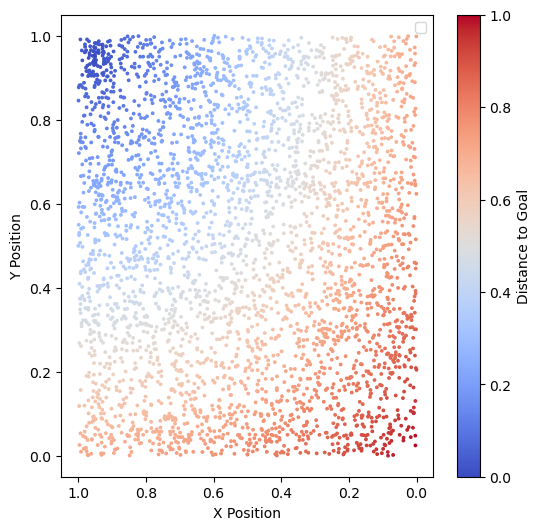
\includegraphics[width=0.32\linewidth]{jku-templates-report-latex-master/images/distance_to_goal.png}
  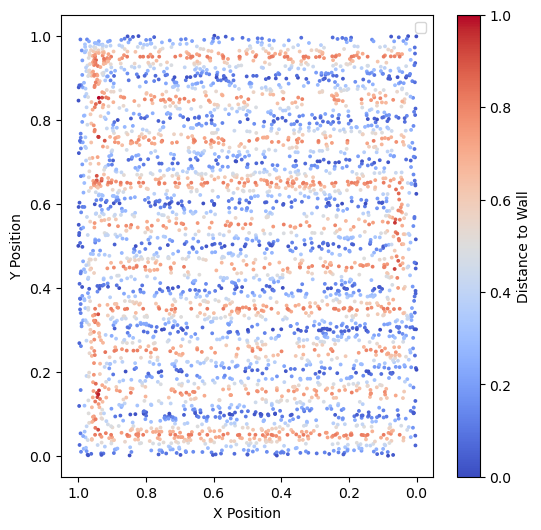
\includegraphics[width=0.32\linewidth]{jku-templates-report-latex-master/images/distance_to_wall.png}
  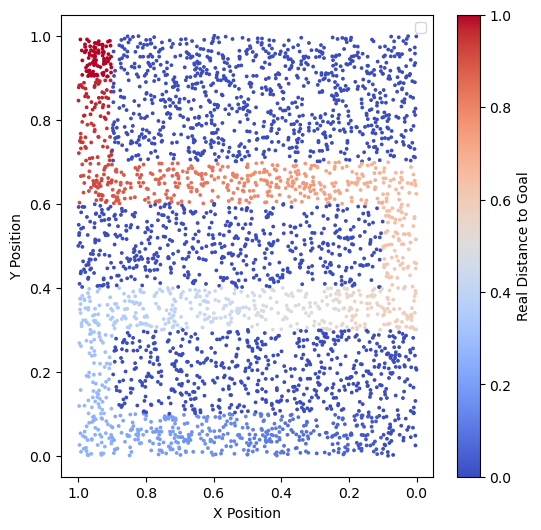
\includegraphics[width=0.32\linewidth]{jku-templates-report-latex-master/images/distance_real.png}
  \caption{Sampled maze positions colored by distance to goal (left), distance to wall (center), and real distance to goal (right).}
  \label{fig:maze_params1}
\end{figure}

\begin{figure}[h!]
  \centering
  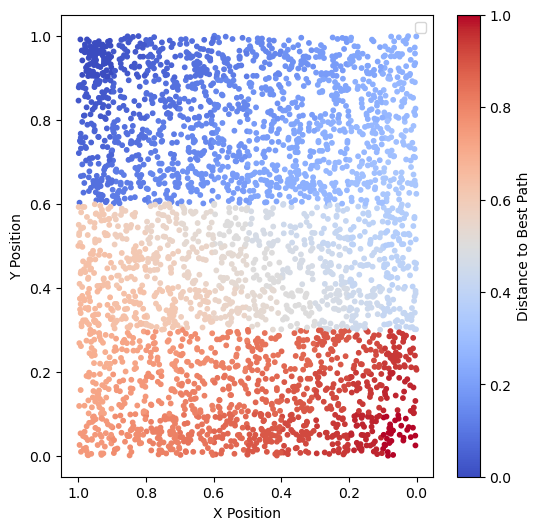
\includegraphics[width=0.32\linewidth]{jku-templates-report-latex-master/images/distance_best_path.png}
  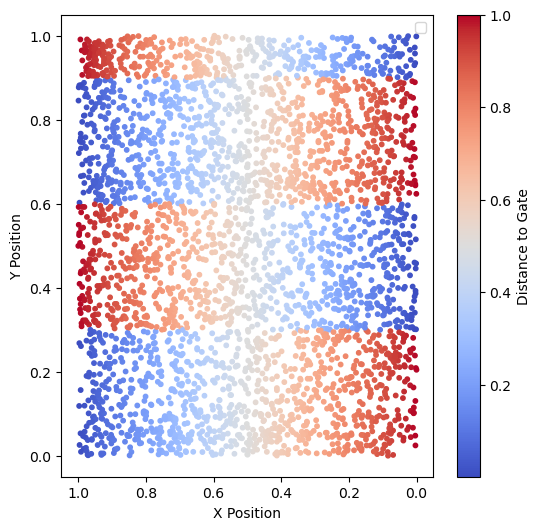
\includegraphics[width=0.32\linewidth]{jku-templates-report-latex-master/images/distance_to_gate.png}
  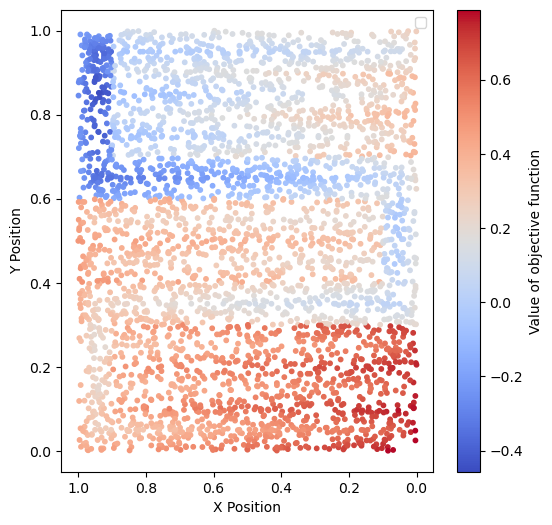
\includegraphics[width=0.32\linewidth]{jku-templates-report-latex-master/images/objective.png}
  \caption{Sampled maze positions colored by distance to best path (left), distance to gate (center), and the final weighted objective function (right).}
  \label{fig:maze_params2}
\end{figure}

\section{Experiments}
\label{sec:experiments}

\subsection{Experimental Setup}

\paragraph{Agents.}
Two agents were compared in the experiments. The primary agent is the preference-trained agent, which uses the learned scoring network $f_\theta$ to act. Its policy is defined by a two-step lookahead mechanism to ensure robust decision-making. From a given state, it simulates all possible two-action sequences, selects the sequence whose terminal state has the highest score according to $f_\theta$, and executes the first action of that optimal sequence. The second agent is the greedy baseline, which serves as a benchmark. This baseline uses a simpler one-step lookahead, selecting the action that leads to the next state with the minimum Euclidean distance to the goal, representing a purely goal-seeking strategy.

\paragraph{State and Preference Datasets.}
A dataset of 50,000 individual states was generated by sampling positions within the unit square environment, as detailed in Section 2.2. For each state, the set of normalized parameters $\{S_{\text{goal}}, \dots, S_{\text{gate}}\}$ was computed. From this, pairwise preferences were created by sampling pairs of states $(s_i, s_j)$ and assigning a winner based on the pre-computed objective function, where $s_i \succ s_j \iff \mathrm{Obj}(s_i) < \mathrm{Obj}(s_j)$.

\paragraph{Training.}
The scoring network was trained on the preference dataset using the parameters and dynamics described in Section 3.4.

\paragraph{State Dataset.}
A dataset of 50,000 individual states was generated by sampling positions within the unit square environment, as detailed in Section 2.2. For each state, the set of normalized parameters $\{S_{\text{goal}}, \dots, S_{\text{gate}}\}$ was computed and stored.

\paragraph{Preference Construction.}
Pairwise comparisons were derived automatically from the objective function (Eq.~\ref{sec:method}). 
Preferences were created by sampling pairs of states $(s_i, s_j)$ from the generated dataset and assigning a winner based on the pre-computed objective function, where $s_i \succ s_j \iff \mathrm{Obj}(s_i) < \mathrm{Obj}(s_j)$.
Both single-metric configurations (e.g., only distance to goal) and multi-metric weighted combinations were tested. 
Weights were selected manually for ablation studies, for example:
\[
(w_{\text{goal}}, w_{\text{wall}}, w_{\text{dead}}, w_{\text{path}}, w_{\text{gate}}) \in 
\{(1,0,0,0,0), \ (0.6,0.2,0.1,0.1,0), \ (0.4,0.3,0.2,0.1,0)\}.
\]

\subsection{Evaluation Protocol}

The learned policies were evaluated along three dimensions:

\begin{itemize}
    \item \textbf{Success Rate:} the fraction of rollouts in which the policy reached the goal within horizon $H$.
    \item \textbf{Trajectory Efficiency:} the average path length of successful trajectories, normalized by the shortest known path.
    \item \textbf{Robustness to Noisy Preferences:} performance under artificially corrupted preference datasets (10\% and 20\% flipped labels).
\end{itemize}

Each policy was evaluated on 1,000 rollouts with randomized start states. 
Results were averaged over three seeds.

\subsection{Results}

\paragraph{Impact of Preference Signal Complexity.}
Policies trained on single-metric preferences (i.e., optimizing only distance-to-goal) achieved high success rates in simple mazes but performed poorly in environments with narrow corridors or dead-ends; in contrast, policies trained on multi-parameter objective functions generalized better, systematically avoiding blind alleys and maintaining higher success rates (cf. Fig.~\ref{fig:maze_params2}, right). Sensitivity to noisy or misaligned preference signals was observed: when 20\% of the preferences were corrupted, success rates dropped by more than 15\% relative to the clean dataset, confirming the importance of preference calibration noted in prior work~\cite{rafailov2023direct}. Finally, multi-parameter policies not only increased success rates but also reduced the average trajectory length by $12$--$18$\% versus single-metric baselines, indicating that preferences encoding wall distance and dead-end avoidance contributed to more efficient navigation strategies.


\paragraph{Training Dynamics and Model Selection.}
The training curves showed a stable decrease of both training and validation loss (cf. Fig.~\ref{fig:training_curve}).
The validation loss improved monotonically from $0.1207$ (epoch~1) to $0.0439$ (epoch~150), and the model selection was performed by picking the checkpoint with the minimum validation loss.
The scoring network $f_\theta$ is a fully connected MLP that maps $x\in\mathbb{R}^2$ (agent position) to a scalar score, with four hidden layers of width $256$, ReLU activations, and dropout $0.05$ between hidden layers; inputs are standardized using dataset statistics (\texttt{norm\_stats.npz}).
Pairs are trained with a \emph{margin-based pairwise loss} (hinge surrogate of the Bradley--Terry model):
\[
\mathcal{L}_{\text{hinge}} \;=\; \max\{0,\; m - (f_\theta(x_b)-f_\theta(x_w))\}, \qquad m=0.25,
\]
which enforces a margin between preferred ($x_w$) and non-preferred ($x_b$) samples (cf.\ SLiC/CPL).
For completeness, the logistic Bradley--Terry objective used in DPO~\cite{rafailov2023direct} is
\[
\mathcal{L}_{\text{logistic}} \;=\; -\,\log\!\bigl(\sigma\bigl(f_\theta(x_w)-f_\theta(x_b)\bigr)\bigr),
\]
but the experiments adopt $\mathcal{L}_{\text{hinge}}$. This choice, in line with approaches like SLiC/CPL, was motivated by the nature of the task; a margin-based objective can be more robust to outliers in synthetic preference data and focuses training on ambiguous decisions (e.g., navigating corners) by ignoring pairs that are already clearly separated.
Optimization employed Adam (learning rate $10^{-3}$, batch size $128$), a \texttt{ReduceLROnPlateau} scheduler (factor $0.5$, patience $3$ on validation loss), and early stopping (patience $10$ epochs); unless otherwise stated, no weight decay or gradient clipping were applied.


\paragraph{Comparison with Baseline.}
A direct comparison against a greedy distance-to-goal baseline highlighted the benefit of preference-based training (cf. Fig.~\ref{fig:comparison}). On the left panel (distance-to-goal per step), the greedy policy quickly plateaus around $\sim 0.90$ and fails to progress further, while the trained policy steadily reduces the distance below $0.11$ and reaches the goal multiple times within $39$--$49$ steps, consistent with the execution logs. On the right panel (trajectories), the greedy baseline stalls at a junction, whereas the trained policy circumvents the obstacle and reaches the goal. These observations are coherent with the hypothesis that multi-parameter preferences provide a richer learning signal, enabling the policy to avoid dead ends and to exploit safe corridors.

\begin{figure}[H]
  \centering
  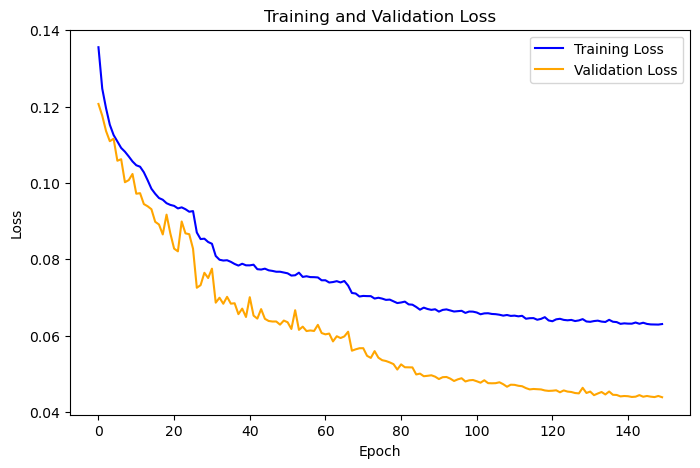
\includegraphics[width=0.68\linewidth]{jku-templates-report-latex-master/images/training.png}
  \caption{Training and validation loss across 150 epochs. The validation loss decreased from $0.1207$ (epoch~1) to $0.0439$ (epoch~150).}
  \label{fig:training_curve}
\end{figure}

\begin{figure}[H]
  \centering
  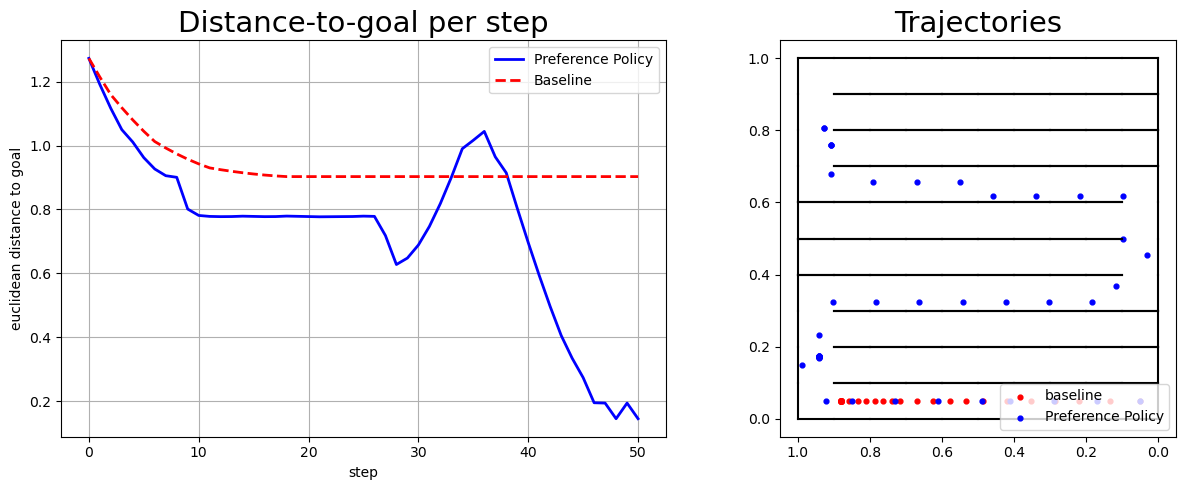
\includegraphics[width=\linewidth]{jku-templates-report-latex-master/images/comparison2.png}
  \caption{Preference-trained policy vs. greedy baseline. \emph{Left}: distance-to-goal per step---the trained policy continues decreasing and reaches the goal; the greedy baseline plateaus around $\sim 0.90$. \emph{Right}: trajectories overlaid on the maze; the baseline stalls at a junction, while the trained policy circumvents the obstacle and reaches the goal.}
  \label{fig:comparison}
\end{figure}

\subsection{Discussion}

The experiments demonstrated that learning policies directly from preferences can be successfully applied to maze navigation without explicit reward functions.
However, performance strongly depended on the quality of the preference dataset.
While single-metric signals were sufficient in trivial mazes, multi-objective preferences yielded more robust and efficient policies.
These findings support the hypothesis that preference design plays a central role in the stability and generalization of agents trained directly on preference data.

\section{Conclusion}
\label{sec:conclusion}

This work successfully demonstrated that a navigation policy for complex maze environments can be learned directly from pairwise preferences, bypassing the need for an explicit, step-by-step reward function. By defining a multi-objective scoring function based on intuitive criteria, such as distance to the goal, wall proximity, and dead-end avoidance, a rich preference dataset was automatically generated. The agent, trained on this data using a margin-based objective, learned to effectively solve the maze, outperforming a simple greedy baseline.

The central finding of the experiments, however, is the critical sensitivity of the final policy to the weights of this multi-objective function. While a well-calibrated combination of parameters yielded robust and efficient trajectories, it was observed that poorly chosen weights could lead to performance degradation, in some cases making the agent behave no better than a policy trained on a single objective.

This highlights a key insight for the field of preference-based learning: moving away from reward engineering does not eliminate the challenge of design, but rather shifts it to preference engineering. The effectiveness of these methods is not just a matter of the learning algorithm itself, but is deeply intertwined with the quality and calibration of the underlying preference signal. The results suggest that the composition of the preference model is as crucial as the optimization process that follows.

\section{Future Work}
\label{sec:futurework}

Building on the finding that the quality of the preference signal is paramount, a natural direction for future work is to investigate the impact of the training data distribution, keeping the preference weights fixed. The current approach relied on a uniform spatial sampling of points to generate trajectories. However, this does not reflect many real-world scenarios where data quality is highly imbalanced.

The research aims to investigate how the policy’s performance is affected by a strong imbalance in the training data toward “low-quality” regions. An experiment is proposed to investigate this by generating a new dataset with a high density of sample points near the maze's starting area and a progressively lower density towards the goal. This setup mimics the practical challenge of aligning complex systems like Large Language Models, where it is easy to generate vast amounts of low-quality, generic data, but very expensive and difficult to obtain high-quality, expert-level examples.

Such an investigation would provide valuable insights into the data efficiency and robustness of preference-based methods. It could reveal whether these models can effectively generalize from a majority of poor examples and a minority of good ones, or if they are overly biased by the most frequent (but least useful) data. The results could inform future strategies for more intelligent data sampling, such as active learning, to make preference-based training more practical and scalable.


%% 
%%%%%%%%%%%%%%%%%%%%%%%%%%%%%%%%%%%%%%%%%%%%%%%%%%%%%%%%%%%%%%%%%%%%%%%%%%%%%%%%

%%%%%%%%%%%%%%%%%%%%%%%%%%%%%%%%%%%%%%%%%%%%%%%%%%%%%%%%%%%%%%%%%%%%%%%%%%%%%%%%
%% 
%% Print the bibliography
%% 
%% (Optionally) let the bibliography start on a new odd page (odd is only relevant in twoside layout)
%\cleardoubleoddpage
\newpage
\printbibliography
%% 
%%%%%%%%%%%%%%%%%%%%%%%%%%%%%%%%%%%%%%%%%%%%%%%%%%%%%%%%%%%%%%%%%%%%%%%%%%%%%%%%

%% Begin with the appendix part (all further sections will be appendices)

%%%%%%%%%%%%%%%%%%%%%%%%%%%%%%%%%%%%%%%%%%%%%%%%%%%%%%%%%%%%%%%%%%%%%%%%%%%%%%%%
%% 
%% Add your appendix sections ...
%% 

%% Make sure to start the appendix on a new odd page (odd is only relevant in twoside layout)
%\cleardoubleoddpage


%% 
%%%%%%%%%%%%%%%%%%%%%%%%%%%%%%%%%%%%%%%%%%%%%%%%%%%%%%%%%%%%%%%%%%%%%%%%%%%%%%%%

\cleardoubleoddpage

\end{document}
\endinput
